\section{Spannungsregler}
  {\bf{Qualit\"atsmasse}}\\
  \begin{minipage}[t]{6cm}
    Ausg.-spannung bestimmt durch:\\
    relativen Stabilisierungsfaktor $S'$\\
    \vspace{0.5mm}{$S' = \frac{\frac{\Delta U_e}{U_e}}{\frac{\Delta U_a}{U_a}}$}
  \end{minipage}
  \begin{minipage}[t]{6cm}
    Temperaturverhalten:\\
    Temperaturkoeffizient $TK_U$\\
    \vspace{0.5mm}{$TK_U = \frac{1}{U_a}\frac{dU_a}{dT}$}
  \end{minipage}
  \begin{minipage}[t]{6cm}
    Lastabh\"angigkeit:\\
    dynamischer Ausgangswiderstand $r_a$\\
    \vspace{0.5mm}{$r_a = \frac{dU_a}{dI_a}$}
  \end{minipage}\\ 
    
\subsection{Linearer Regler}
  \begin{minipage}[T]{14cm}
    Ausgangsspannung
    \hspace{13mm}\fbox{$V_{out} = \left(1+\frac{R_1}{R_2}\right) \cdot V_{ref}$}\\
  \end{minipage}
  \begin{minipage}{5cm}
    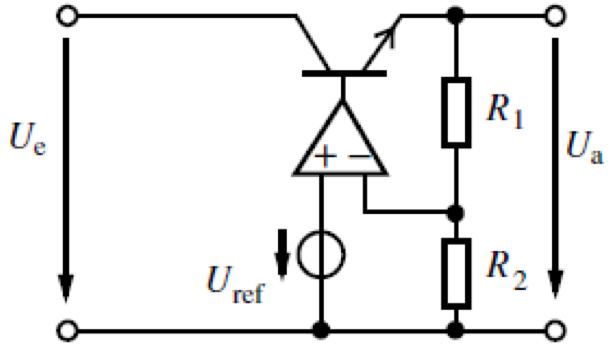
\includegraphics[height=1.5cm]{./bilder/ReglerLinear.png}
  \end{minipage}\\
            
\subsection{Einstellbarer Regler}
  \begin{minipage}[T]{14cm}
    Ausgangsspannung
    \hspace{13mm}\fbox{$V_{out} = V_{ref} + R_2 \cdot\left(\frac{V_{ref}}{R_1} + I_{adj}\right)  \approx\left(1+\frac{R_2}{R_1}\right) 
    \cdot V_{ref}$}\\
  \end{minipage}
  \begin{minipage}{5cm}
    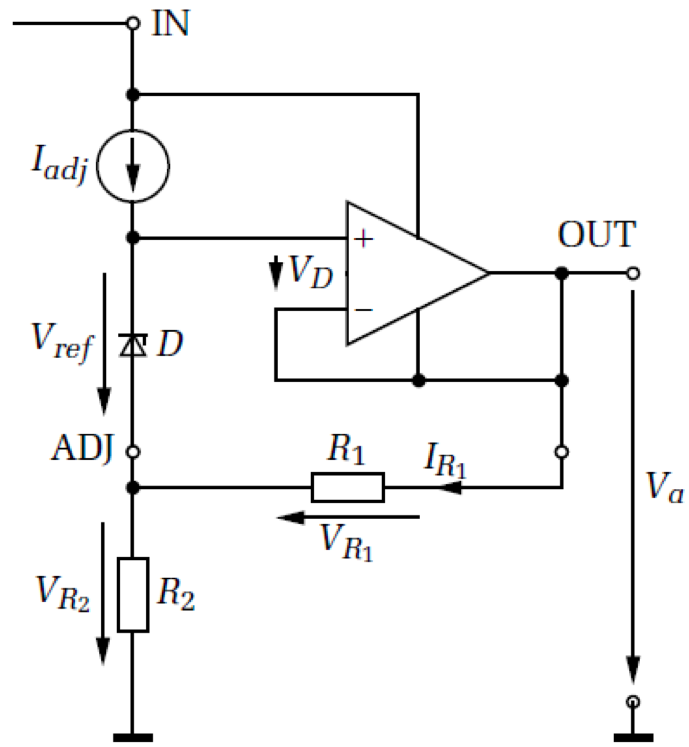
\includegraphics[height=2.5cm]{./bilder/ReglerEinstellbar.png}
  \end{minipage}\\
        
\subsection{Aufw\"artswandler (Step up, Boost)}
  \begin{minipage}[T]{14cm}
    Lade-Phase (S geschlossen)
    \hspace{0.5mm}\fbox{$\Delta I_{L\_on} = \frac{1}{L}V_{in}\cdot t_{on}$}\\  
    Entlade-Phase (S offen)
    \hspace{5.8mm}\fbox{$\Delta I_{L\_off} = \frac{1}{L}(V_{in}-V_{out})\cdot t_{off}$}\\  
    Gleichgewicht
    \hspace{21mm}\fbox{$\Delta I_{L\_on} =-\Delta I_{L\_off}$}\\  
    Ausgangsspannung
    \hspace{13mm}\fbox{$V_{out} = V_{in}\cdot \left(1+\frac{t_{on}}{t_{off}}\right)$}\\
  \end{minipage}
  \begin{minipage}{5cm}
    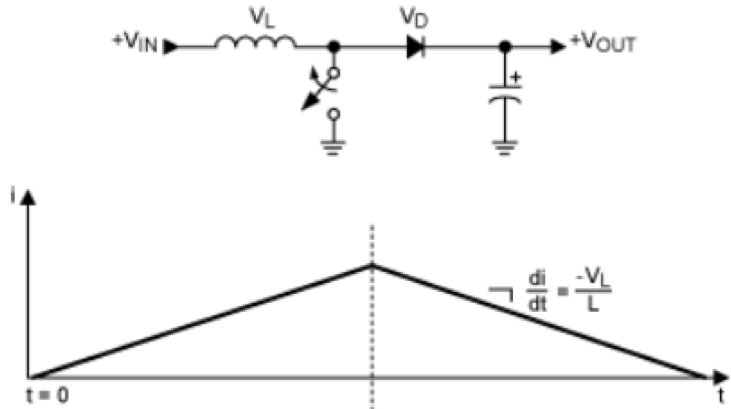
\includegraphics[width=4cm]{./bilder/ReglerStepUpStromverlauf.png}
  \end{minipage}\\
        
\subsection{Abw\"artswandler (Step Down, Buck)}
  \begin{minipage}[T]{14cm}
    Lade-Phase (S geschlossen)
    \hspace{0.5mm}\fbox{$\Delta I_{L\_on} = \frac{1}{L}\int_{0}^{T_i}{(V_{in}-V_{out})dt} = \frac{1}{L}(V_{in}-V_{out})\cdot T_i$}\\  
    Entlade-Phase (S offen)
    \hspace{5.8mm}\fbox{$\Delta I_{L\_off} = \frac{1}{L}\int_{T_i}^{T_S}{(V_{out}+V_{D_f})dt}= \frac{1}{L}(V_{out}+V_{D_f})(T_S-T_i)$}\\
    Ausgangsspannung
    \hspace{13mm}\fbox{$V_{out} = \frac{T_i}{T_S}\cdot V_{in} - \left(1-\frac{T_i}{T_S}\right) \cdot V_{D_f} \approx \frac{T_i}{T_S}
    \cdot V_{in}$}\\
  \end{minipage}
  \begin{minipage}{5cm}
    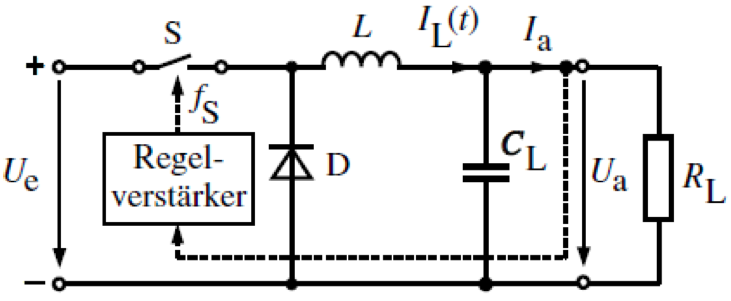
\includegraphics[width=5cm]{./bilder/ReglerStepDown.png}
  \end{minipage}\\
        
\subsection{Invertierender Wandler (Buck-Boost)}
  \begin{minipage}[T]{8cm}
    Ausgangsspannung
    \hspace{13mm}\fbox{$V_{out} = -\frac{T_i}{T_S}\cdot V_{in}$}\\
  \end{minipage}
  \begin{minipage}{6cm}
    $T_i$ = Einschaltzeit\\
    $T_s$ = Ausschaltzeit
  \end{minipage}
  \begin{minipage}{5cm}
    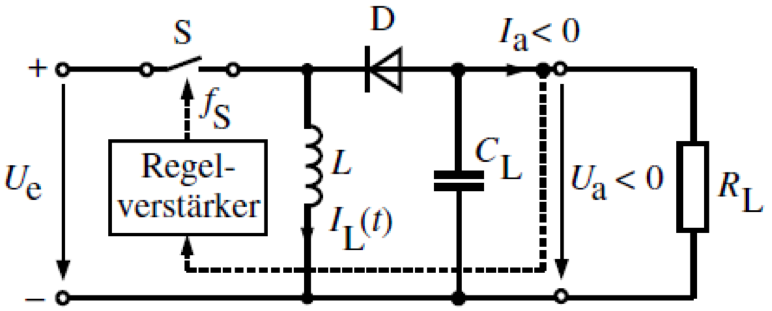
\includegraphics[width=4cm]{./bilder/ReglerInvert.png}
  \end{minipage}\\
        
\subsection{Ladepumpen (Charge-Pumps)}
  \begin{minipage}[T]{14cm}
    \hspace*{43.3mm}\fbox{$\Delta V_{out} = \frac{\Delta Q_1}{C_1+C_L} = \frac{C_1(V_{in}-V_{out})}{C_1+C_L} = \frac{V_{in}-V_{out}}{1+
    \frac{C_L}{C_1}}$}\\
    \hspace*{43.3mm}\fbox{$\Delta Q = C_L \cdot \Delta V_{out} = \frac{C_1 C_L}{C_1+C_L}(V_{in}-V_{out})$}\\
    \hspace*{43.3mm}\fbox{$I_{out} = \frac{\Delta Q}{T_S} = \frac{C_1 C_L}{C_1+C_L}\frac{V_{in}-V_{out}}{T_S}$}\\
    \hspace*{43.3mm}Ver\"anderung der Ausgangsspannung durch ver\"andern der\\
    \hspace*{43.3mm}Schaltfrequenz
  \end{minipage}
  \begin{minipage}{5cm}
    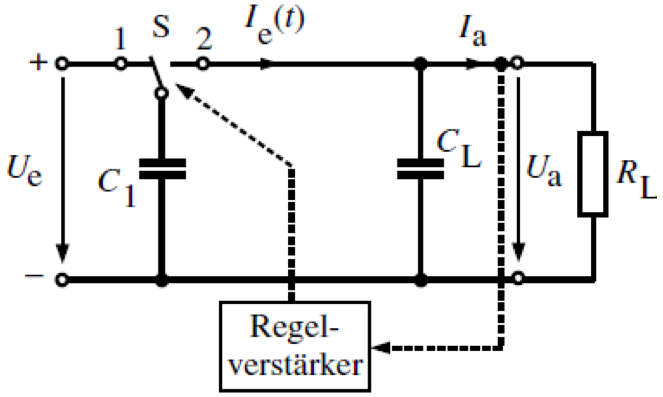
\includegraphics[width=5cm]{./bilder/ReglerChargePump.png}
  \end{minipage}\\  
    
\newpage

\subsection{Wichtiges zu Spule / Kondensator}
  Energie im Mag.-Feld
  \hspace{9mm}\fbox{$W_m = \frac{1}{2} \cdot L \cdot I^2 = \frac{1}{2}\cdot N \cdot I \cdot \Phi$}\\
  Energie im El.-Feld
  \hspace{12.5mm}\fbox{$W_E = \underbrace{\frac{1}{2} \cdot C \cdot U^2}_{U = konst}  = \frac{1}{2} \cdot Q \cdot U = \underbrace{\frac{1}{2}
  \cdot\frac{Q^2}{C}}_{Q = konst}$}\\
  Spule
  \hspace{34mm}\fbox{$u_L(t) = L \cdot \frac{di(t)}{dt}$}\\
  \hspace*{43.5mm}\fbox{$i_L(t) = \frac{1}{L}\int\limits_0^t u(\tau)d\tau + i(0)$}\\
  Kondensator
  \hspace{22.7mm}\fbox{$u_C(t) = \frac{1}{C}\int\limits_0^t i(\tau)d\tau + u(0)$}\\
  \hspace*{43.5mm}\fbox{$i_C(t) = C \cdot \frac{du(t)}{dt}$}\\
     